\chapter{Estado del arte}

En este capítulo se hace un repaso de las distintas soluciones que existen actualmente para la creación de bots de \textit{Discord} y la configuración de sus comandos.

\section{Contexto y definiciones previas}

Los bots actúan como un usuario más dentro de un servidor de \textit{Discord}. En cambio, debido a su naturaleza, deben ser agregados a los servidores por usuarios humanos. Se pueden crear infinidad de bots, por lo que han surgido páginas web (como \href{https://top.gg/}{top.gg} o \href{https://bots.ondiscord.xyz/}{Bots on Discord}) que permiten que los usuarios encuentren bots ya creados y desplegados listos para ser utilizados en sus servidores. Estos cuentan con funcionalidades específicas, por lo que no pueden modificarse por los usuarios.

Además de este tipo de bots y webs, han surgido otras plataformas que permiten que los usuarios creen y configuren sus propios bots. Estas son las que se desarrollan en este capítulo. A continuación se enumeran algunos conceptos que son interesantes conocer ya que se utilizan tanto en este capítulo como en el resto del documento.

Conceptos técnicos, que definen la manera en la que se estructuran, configuran y definen los bots:

\begin{itemize}
	\item \textbf{Comandos predefinidos}. Comandos cuya funcionalidad está ya definida (y por tanto programada) y no puede ser modificada por un usuario.
	\item \textbf{Comandos personalizados}. Comandos que se pueden crear a partir de comandos predefinidos que pueden utilizarse con distintos parámetros para modificar su comportamiento.
	\item \textbf{Comandos reutilizables}. Comandos personalizados que una vez configurados pueden utilizarse en distintos bots.
	\item \textbf{Despliegue de un bot}. Todas aquellas tareas y actividades que hacen que un bot se encuentre disponible para ser usado por usuarios.
	\item \textbf{Control del despliegue}. Capacidad de controlar y monitorizar el despliegue de bots en un sistema.
\end{itemize}

Conceptos relacionados con funcionalidades de \textit{Discord}:

\begin{itemize}
    \item \textbf{Comandos de moderación}. Comandos cuya funcionalidad se centra en la moderación de usuarios en los servidores de \textit{Discord}.
\end{itemize}

\section{Soluciones actuales}

Las soluciones actuales se podrían dividir en dos grupos, las herramientas \textit{no-code} y aquellas herramientas que hacen uso de programación. En ambas la interacción con el sistema se hace a través de una aplicación web y, además, suelen tener una apariencia muy similar, siendo las \textit{no-code} algo más complejas de usar. Las primeras se centran en usuarios con menor conocimiento técnico, abstrayendo todos los detalles de este tipo. En cambio, las segundas son utilizadas por aquellos usuarios con un conocimiento informático más amplio.

En las siguientes secciones se incluyen las herramientas con características más interesantes. Por otro lado, para cada herramienta se incluye una tabla como la siguiente, donde se resumen las características más importantes de cada una de ellas.

\FloatBarrier
\begin{table}[h]
    \centering
    \def\arraystretch{1.25}
    \begin{adjustbox}{max width=\textwidth}
    \begin{tabularx}{325px}{|l|L|}
    \hline
        \multicolumn{2}{|c|}{\textbf{Nombre de la herramienta}} \\ \hline
    \hline
        \textbf{Tipo de comandos} & El tipo de comandos que provee la herramienta, y la cantidad de comandos personalizados que se pueden crear. \\ \hline
        \textbf{Comandos reutilizables} & Si los comandos se pueden reutilizar entre bots o no. \\ \hline
        \textbf{Control del despliegue} & Si el usuario tiene control del despliegue del bot o no. \\ \hline
        \textbf{Número de bots} & La cantidad de bots que el usuario puede crear y configurar. \\ \hline
        \textbf{Experiencia} & La experiencia de usuario a la hora de utilizar las herramientas. \\ \hline
        \textbf{Personalización extra} & Si la herramienta permite una personalización más avanzada, y si es de pago o no. \\ \hline
        \textbf{Características} & Las funcionalidades configurables en los bots. \\ \hline
        \textbf{Logs} & Si permiten que los usuarios tengan acceso a los logs de los bots. \\ \hline
        \textbf{Premium} & Coste de los planes de pago de la herramienta. \\ \hline
    \end{tabularx}
    \end{adjustbox}
    \caption{Cuadro resumen de las características de una herramienta.}
\end{table}
\FloatBarrier

\subsection{Herramientas \textit{no-code}}

Estas herramientas permiten la creación de bots sin hacer uso de recursos de programación o similares. Cuentan con un repertorio de comandos predefinidos, de los cuales se pueden crear comandos personalizados modificando los parámetros de estos. Esto se hace a través de interfaces gráficas sencillas compuestas por formularios y otros elementos.

Por ejemplo, el comando predefinido más común sirve para enviar mensajes. A partir de este comando se pueden crear distintos comandos personalizados, cambiando la palabra clave que los usuarios deben introducir (en los canales de texto) para activar el comando y el mensaje que el bot debe enviar.

En general la mayoría tienen una serie de funcionalidades gratuitas, teniendo que suscribirse a un plan de pago mensual para obtener funcionalidades extra. Estas suscripciones suelen tener un coste aproximado de cinco dólares mensuales, pudiendo comprar suscripciones anuales o incluso de por vida y suelen ofrecer un repertorio de comandos más amplio, conexiones con redes sociales, estadísticas de uso e incluso \textit{logging}.

En la mayoría de casos estas plataformas cuentan con un único bot que se debe agregar al servidor de \textit{Discord} deseado. Esto implica que el uso de estos servicios no permite por tanto agregar varios bots con distintas funcionalidades a un mismo servidor. Si un usuario utiliza \textit{ProBot} (servicio que se explica en detalle a continuación), entonces el bot que proporciona \textit{ProBot} sólo podrá utilizarse una sola vez por servidor.

En ellas se puede observar también uno de los principales problemas ya mencionados, la muy reducida personalización y reutilización de los comandos. En estos sistemas no se puede crear un comando específico con una funcionalidad concreta, sino que se basan en funcionalidades predefinidas no reutilizables.

Estas funcionalidades predefinidas son en su mayoría de moderación de usuarios y envío de mensajes, y no se pueden reutilizar entre distintos bots. Además, debido a la estructura y arquitectura de estas plataformas, los usuarios no pueden ampliar el repertorio de comandos, teniendo que conformarse con los existentes.

\subsubsection{\textit{ProBot}}

\href{https://probot.io/}{\textit{ProBot}} es sin duda la más interesante de las herramientas \textit{no-code} debido a que permite crear ilimitados comandos personalizados, siendo la principal desventaja que estos comandos son predefinidos, y no se puede cambiar su funcionalidad. Los comandos predefinidos se centran en moderación y mensajes automáticos, por lo que las posibilidades no son muy amplias.

A favor de esta herramienta también destaca que es sencilla de utilizar, la interfaz web intenta imitar a la de \textit{Discord} y es intuitiva. Por contra, es bastante intrusiva la modalidad \textit{premium}, ya que muchas secciones sugieren la compra de esta modalidad. Además es imposible controlar el despliegue del bot, y no es posible reutilizar comandos.

Sus características son:

\FloatBarrier
\begin{table}[h]
    \centering
    \def\arraystretch{1.25}
    \begin{adjustbox}{max width=\textwidth}
    \begin{tabularx}{325px}{|l|L|}
    \hline
        \multicolumn{2}{|c|}{\textbf{\textit{ProBot}}} \\ \hline
    \hline
        \textbf{Tipo de comandos} & Predefinidos (ilimitados) \\ \hline
        \textbf{Comandos reutilizables} & No \\ \hline
        \textbf{Control del despliegue} & No \\ \hline
        \textbf{Número de bots} & 1, único \\ \hline
        \textbf{Experiencia} & Sencilla \\ \hline
        \textbf{Personalización extra} & Requiere \textit{premium} (mensualidades) \\ \hline
        \textbf{Características} & Moderación, estadísticas, mensajes automáticos, música \\ \hline
        \textbf{Logs} & No \\ \hline
        \textbf{Premium} & \$60 al año \\ \hline
    \end{tabularx}
    \end{adjustbox}
    \caption{Características de \textit{ProBot}.}
\end{table}
\FloatBarrier

\FloatBarrier
\begin{figure}[h]
	\centering
	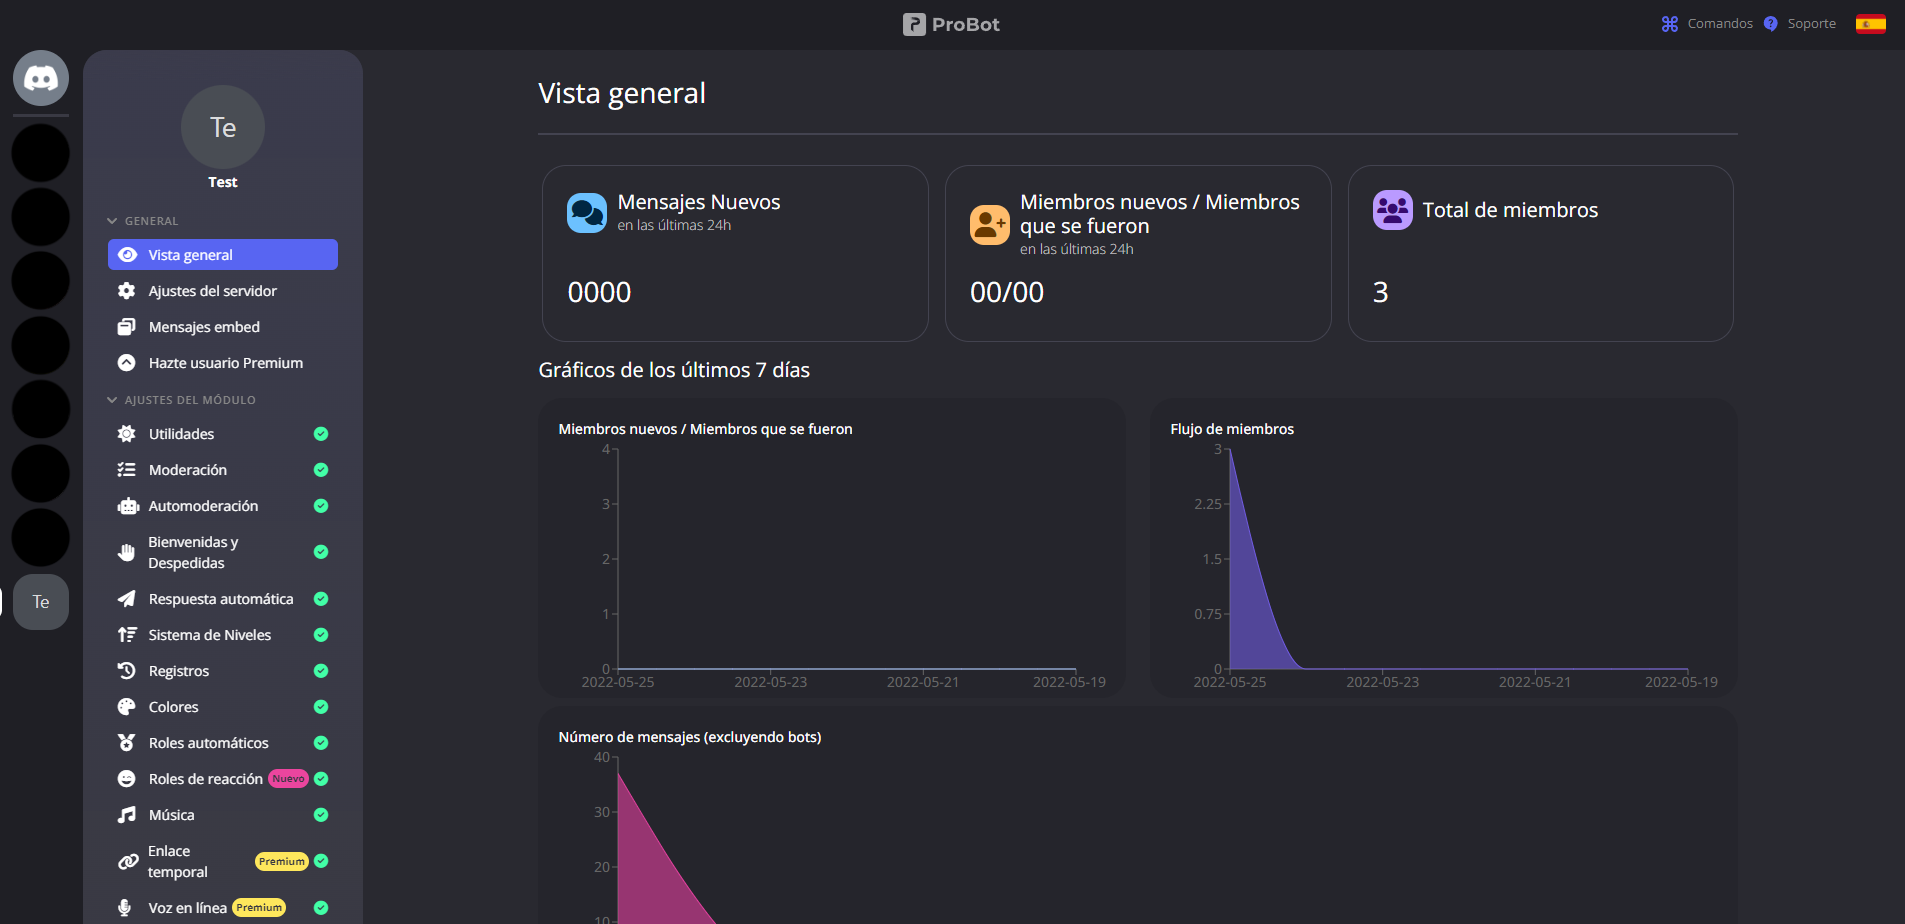
\includegraphics[width=1\textwidth]{img/probot.png}
	\caption{Interfaz web de \textit{ProBot}.}
\end{figure}
\FloatBarrier

\subsubsection{\textit{Mee6}}

\href{https://mee6.xyz/}{\textit{Mee6}} es otra herramienta muy similar a la anterior, siendo la principal diferencia que en este caso los comandos personalizados se limitan a 5. Por contra, tiene un mayor catálogo de funcionalidades.

De nuevo no es posible controlar el despliegue del bot, como tampoco es posible crear otro bot y agregarlo a un mismo servidor, o reutilizar comandos.

Sus características son:

\FloatBarrier
\begin{table}[h]
    \centering
    \def\arraystretch{1.25}
    \begin{adjustbox}{max width=\textwidth}
    \begin{tabularx}{325px}{|l|L|}
    \hline
        \multicolumn{2}{|c|}{\textbf{\textit{Mee6}}} \\ \hline
    \hline
        \textbf{Tipo de comandos} & Predefinidos (muy limitados, 5) \\ \hline
        \textbf{Comandos reutilizables} & No \\ \hline
        \textbf{Control del despliegue} & No \\ \hline
        \textbf{Número de bots} & 1, único \\ \hline
        \textbf{Experiencia} & Sencilla \\ \hline
        \textbf{Personalización extra} & Requiere \textit{premium} (mensualidades) \\ \hline
        \textbf{Características} & · Moderación, estadísticas, mensajes automáticos, música, temporizadores, \textit{quiz} / \textit{trivia} \\ \hline
        \textbf{Logs} & No \\ \hline
        \textbf{Premium} & \$50 al año / \$90 de por vida  \\ \hline
    \end{tabularx}
    \end{adjustbox}
    \caption{Características de \textit{Mee6}.}
\end{table}
\FloatBarrier

\FloatBarrier
\begin{figure}[h]
	\centering
	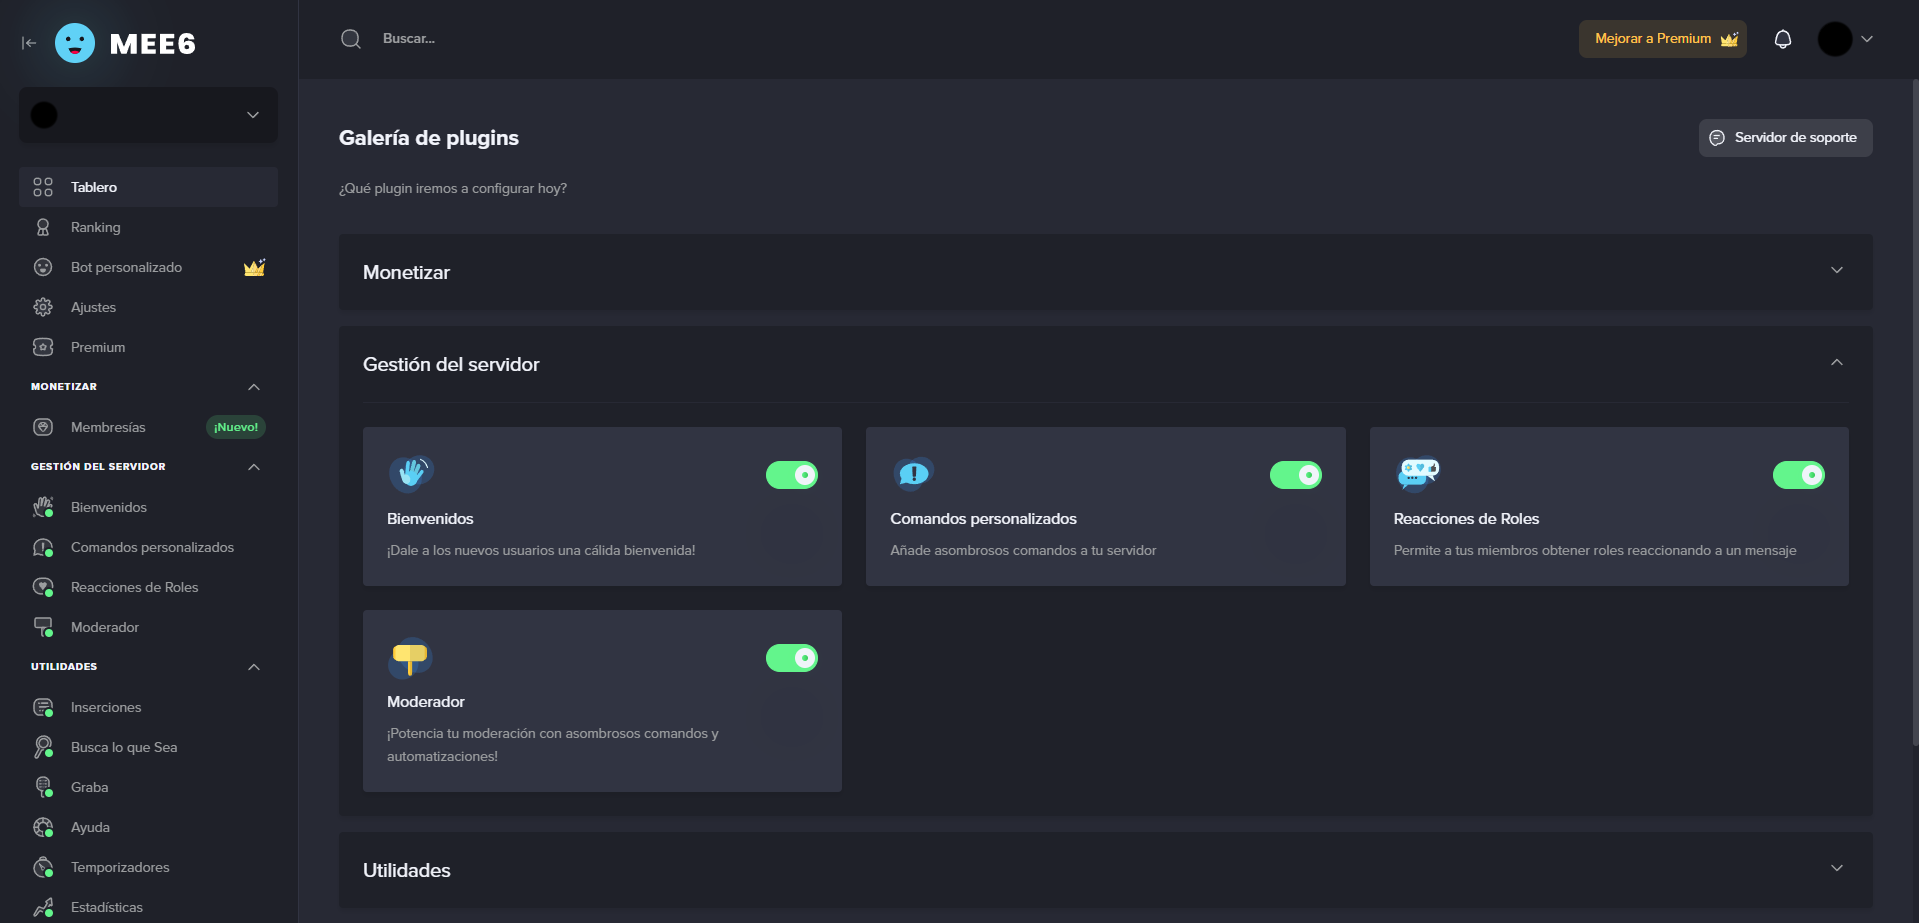
\includegraphics[width=1\textwidth]{img/mee6.png}
	\caption{Interfaz web de \textit{Mee6}.}
\end{figure}
\FloatBarrier


\subsubsection{\textit{BotGhost}}

\href{https://botghost.com/}{\textit{BotGhost}} es un híbrido entre \textit{ProBot} y \textit{Mee6}, ya que tiene características comunes de ambos. La principal característica de esta herramienta es que permite crear comandos personalizados haciendo uso de una serie de módulos que se pueden interconectar para definir el ciclo de vida de un comando.

Esta característica es muy interesante, pero está muy limitada y las funcionalidades que permite realizar se resumen en envío de mensajes y tareas de moderación de usuarios muy básicas. El plan \textit{premium} sería necesario en este caso para poder sacarle partido a esta funcionalidad.

Otro aspecto interesante es que se pueden crear distintos bots, hasta 50 distintos si se opta por la opción \textit{premium}. Sus características son las siguientes.

\FloatBarrier
\begin{table}[h]
    \centering
    \def\arraystretch{1.25}
    \begin{adjustbox}{max width=\textwidth}
    \begin{tabularx}{325px}{|l|L|}
    \hline
        \multicolumn{2}{|c|}{\textbf{\textit{BotGhost}}} \\ \hline
    \hline
        \textbf{Tipo de comandos} & Predefinidos (muy limitados, 5) \\ \hline
        \textbf{Comandos reutilizables} & Sí \\ \hline
        \textbf{Control del despliegue} & No (Sólo encendido y apagado) \\ \hline
        \textbf{Número de bots} & 1, único (50 con \textit{premium}) \\ \hline
        \textbf{Experiencia} & Compleja \\ \hline
        \textbf{Personalización extra} & Requiere \textit{premium} (mensualidades) \\ \hline
        \textbf{Características} & · Moderación, estadísticas, mensajes automáticos, temporizadores, integración con videojuegos, meteorología, música, \textit{quiz} / \textit{trivia} \\ \hline
        \textbf{Logs} & No \\ \hline
        \textbf{Premium} & \$60 al año / \$100 de por vida \\ \hline
    \end{tabularx}
    \end{adjustbox}
    \caption{Características de \textit{BotGhost}.}
\end{table}
\FloatBarrier

\FloatBarrier
\begin{figure}[h]
	\centering
	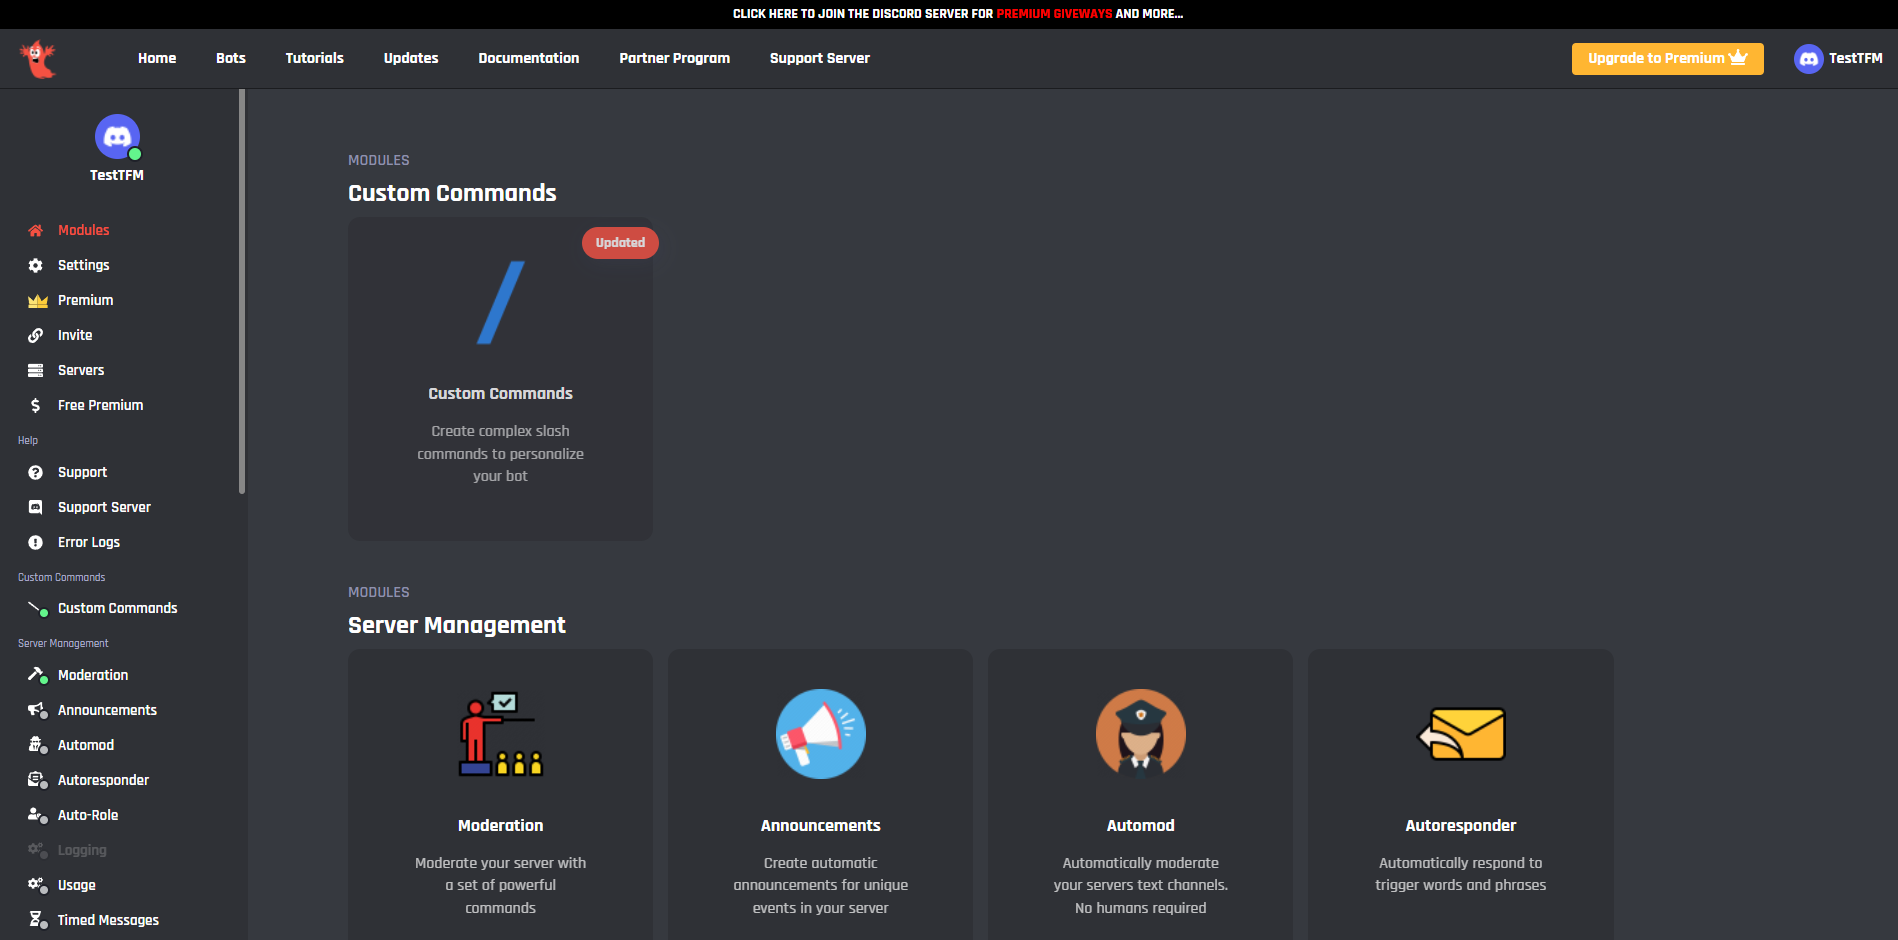
\includegraphics[width=1\textwidth]{img/botghost.png}
	\caption{Interfaz web de \textit{BotGhost}.}
\end{figure}
\FloatBarrier

\subsection{Herramientas de programación}

Actualmente existen multitud de librerías para distintos lenguajes de programación que permiten interactuar con la \textit{API} de \textit{Discord} y por tanto crear un bot. Así mismo existen herramientas híbridas que permiten esta creación de una manera más sencilla.

\subsubsection{\textit{Autocode}}

\href{https://autocode.com/}{\textit{Autocode}} es sin duda la herramienta mas interesante que existe de esta modalidad híbrida. Realmente es una plataforma que facilita la creación y despliegue de aplicaciones y servicios web, bots, y tareas de automatización permitiendo que los usuarios escriban sólo una parte del código (\textit{JavaScript}) de estos. Esta plataforma provee al usuario con un editor de código sencillo y de un explorador de archivos, recursos con los cuales puede crear el código.

De este modo el usuario sólo tiene que preocuparse por el código de la aplicación (o bot en este caso) que quiere crear, ya que del despliegue se encarga \textit{Autocode}. En su plan gratuito se pueden crear hasta 50 aplicaciones distintas, y permite la integración entre si de los distintos recursos que el usuario crea en la plataforma.

Sus características son:

\FloatBarrier
\begin{table}[h]
    \centering
    \def\arraystretch{1.25}
    \begin{adjustbox}{max width=\textwidth}
    \begin{tabularx}{325px}{|l|L|}
    \hline
        \multicolumn{2}{|c|}{\textbf{\textit{Autocode}}} \\ \hline
    \hline
        \textbf{Tipo de comandos} & Predefinidos + \textit{JS} \\ \hline
        \textbf{Comandos reutilizables} & No \\ \hline
        \textbf{Control del despliegue} & Sí (limitado) \\ \hline
        \textbf{Número de bots} & 50 gratis \\ \hline
        \textbf{Experiencia} & Algo complejo \\ \hline
        \textbf{Personalización extra} & Requiere \textit{premium} (mensualidades) \\ \hline
        \textbf{Especialidad} & Despliegue general de aplicaciones \\ \hline
        \textbf{Logs} & Sí (1-30 días) \\ \hline
        \textbf{Premium} & \$180 / \$1620 al año \\ \hline
    \end{tabularx}
    \end{adjustbox}
    \caption{Resumen de soluciones actuales.}
\end{table}
\FloatBarrier

\FloatBarrier
\begin{figure}[h]
	\centering
	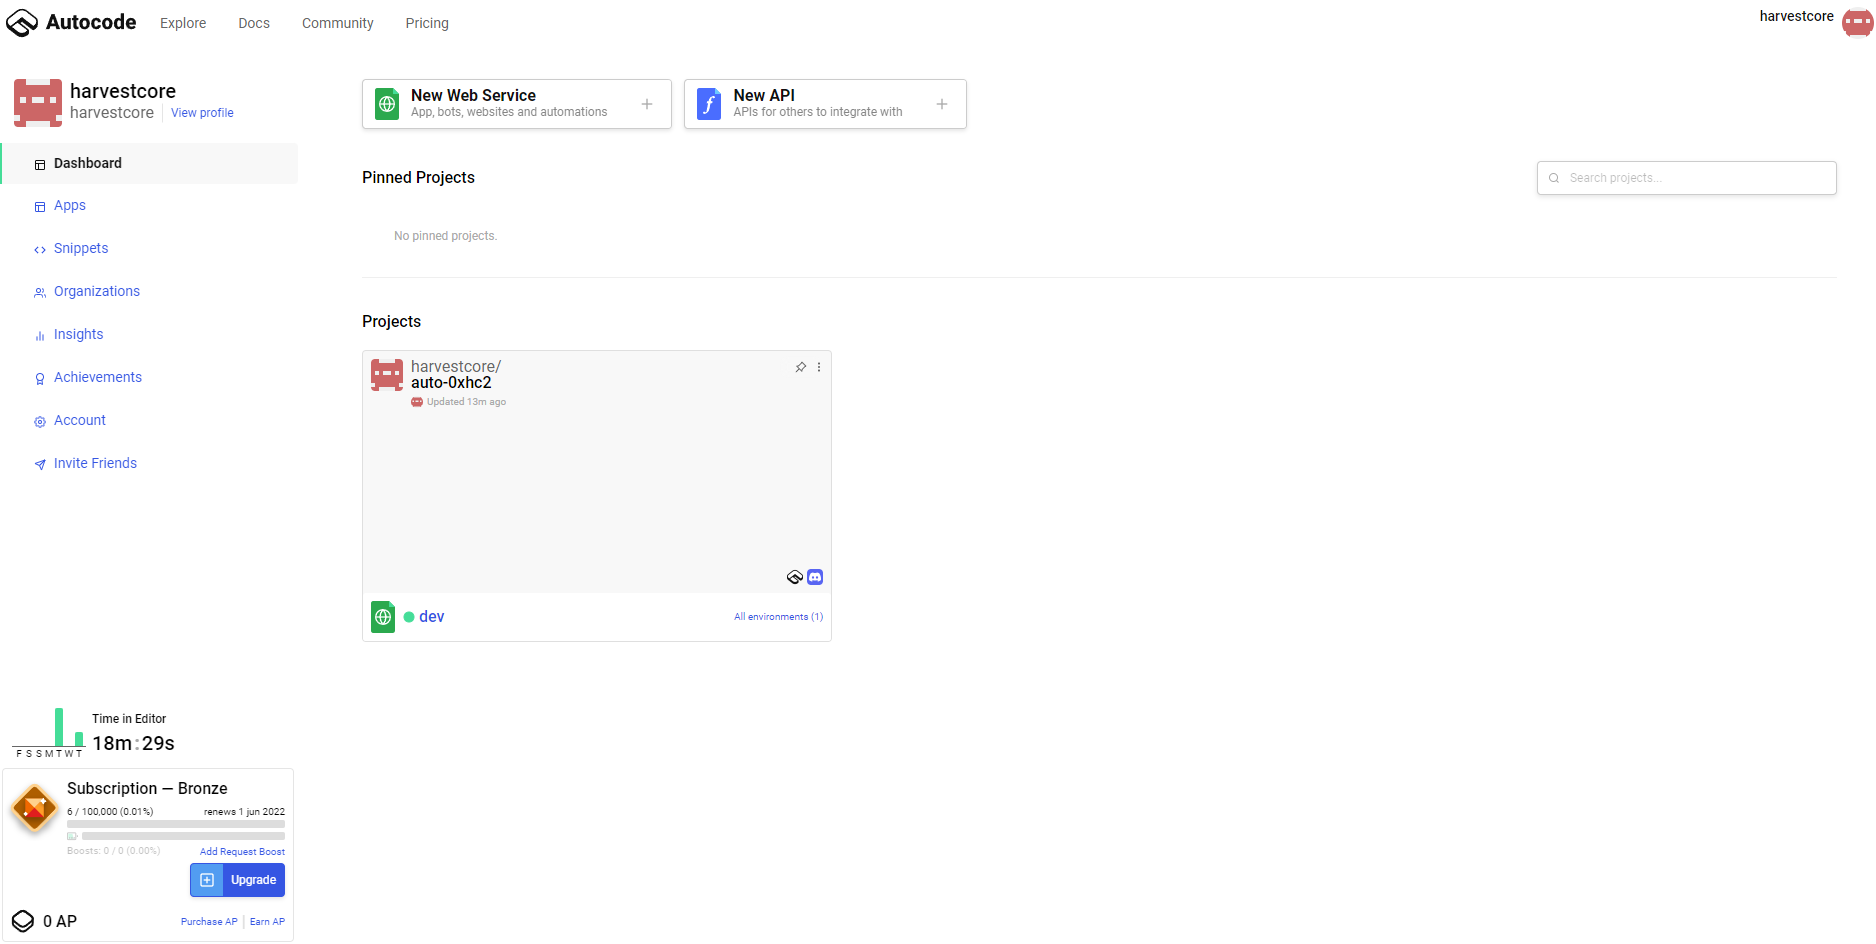
\includegraphics[width=1\textwidth]{img/autocode.png}
	\caption{Interfaz web de \textit{Autocode}.}
\end{figure}
\FloatBarrier

\subsubsection{Librerías de programación}

Las librerías de programación dan libertad total a la hora de crear un bot de \textit{Discord}, lo cual puede ser ideal en algunos casos. Las ventajas son obvias, ya que se puede crear cualquier tipo de comando y la reutilización es sencilla, pero en cambio, la gestión del despliegue puede ser compleja.

Por lo general todas las librerías permiten realizar casi las mismas funcionalidades, diferenciándose en aspectos como el rendimiento, la comunidad que las soporta o la facilidad de uso.

Algunos ejemplos de librerías son:

\begin{itemize}
	\item \textbf{\textit{C\#}}: \href{https://discordnet.dev/}{\textit{Discord.NET}}, \href{https://github.com/DSharpPlus/DSharpPlus}{\textit{DSharpPlus}}
	\item \textbf{\textit{Java}}: \href{https://github.com/DV8FromTheWorld/JDA}{\textit{JDA}}, \href{https://discord4j.com/}{\textit{Discord4J}}
	\item \textbf{\textit{C++}}: \href{https://dpp.dev/}{\textit{D++}}
	\item \textbf{\textit{JavaScript}}: \href{https://discord.js.org/}{\textit{discord.js}}
	\item \textbf{\textit{Golang}}: \href{https://github.com/bwmarrin/discordgo}{\textit{DiscordGo}}
	\item \textbf{\textit{Ruby}}: \href{https://github.com/shardlab/discordrb}{\textit{discordrb}}
\end{itemize}


\subsection{Comparativa de tiempos}

En esta sección se hace una comparativa del tiempo medio de desarrollo desde cero de un bot de \textit{Discord} usando las herramientas anterior mencionadas. Además se incluye tiempos de desarrollo usando tres lenguajes de programación: \textit{C\#}, \textit{JavaScript} y \textit{Python}.

Las mediciones incluyen todos los pasos necesarios para crear uno de estos bots con dos comandos personalizados. En el caso de las herramientas de programación se incluye desde la creación del proyecto hasta el despliegue (en local) de este.

Los dos comandos personalizados se han elegido al ser comunes en todas las plataformas mencionadas, además de sencillos de implementar. Son los siguientes:

\begin{itemize}
	\item Envío de un mensaje.
	\item Envío de un mensaje recurrente (cada cierto tiempo).
\end{itemize}

\FloatBarrier
\begin{table}[h]
    \centering
    \def\arraystretch{1.25}
    \begin{adjustbox}{max width=\textwidth}
    \begin{tabularx}{200px}{|l|R|}
    \hline
        \textbf{Herramienta} & \textbf{Tiempo (en minutos)} \\ \hline
    \hline
        ProBot & 5 \\ \hline
        Mee6 & 5 \\ \hline
        BotGhost & 10 \\ \hline
    \hline
        Autocode (JS) & 45 \\ \hline
    \hline
        JS & 85 \\ \hline
        C\# & 100 \\ \hline
        Python & 80 \\ \hline
    \end{tabularx}
    \end{adjustbox}
    \caption{Comparativa de tiempos de las distintas herramientas analizadas.}
\end{table}
\FloatBarrier

\section{Discusión}

Como se puede observar existen multitud de posibilidades a la hora de crear un bot de \textit{Discord}, y, aunque cumplen lo que prometen, se centran en aspectos muy concretos dejando otros bastante desatendidos.

En las herramientas \textit{no-code} los bots se centran principalmente en tareas de moderación, envío de mensajes, estadísticas e integración con videojuegos y redes sociales. Además, para sacarles partido es necesario el uso de los paquetes \textit{premium}, dejando de lado en el plan gratuito detalles específicos (y que serían ideales) como:

\begin{itemize}
	\item Reutilización de comandos.
	\item Creación de comandos con funcionalidad específica.
	\item Control del despliegue de los bots.
	\item Creación de distintos bots con distintas funcionalidades en un mismo sistema.
\end{itemize}

En el caso de las librerías de programación, aunque todas permiten el acceso a la \textit{API} de \textit{Discord}, cada una de ellas tiene una estructura distinta y los procedimientos para crear un bot o comandos son más o menos complejos. Si un usuario decidiese utilizarlas tendría flexibilidad completa a la hora de crear una estructura concreta, pero entonces tendría que dedicar en ese caso un tiempo necesario para diseñar algo funcional.

\textit{Autocode} es una buena alternativa a las soluciones anteriores, ya que se evita el tener que gestionar el despliegue de los bots y se eliminan algunas trabas de gestión del código, pero al igual que el uso de librerías toda la lógica recae en el usuario final. Esto puede ser útil en ciertos casos, pero no siempre.

En la comparativa de tiempos anterior se puede observar que las herramientas \textit{no-code} son las más rápidas. Esto se debe a que solo es necesario agregar el bot al servidor de \textit{Discord} deseado, y tras eso configurar de manera sencilla los comandos.

En menos de 10 minutos se puede incluir una gran cantidad de funcionalidad a un servidor de \textit{Discord} de manera gratuita, algo que puede ser muy útil para la basta mayoría de usuarios de \textit{Discord}, pero cuando se necesitan funcionalidades específicas entonces no es el sistema ideal.

En cambio, cuando se usan herramientas que hacen uso de código, el tiempo de implementación se incrementa considerablemente. No hace justicia la comparativa, ya que en este caso se tiene que desarrollar el software por completo, por lo que es obvio que el tiempo es mayor.

En definitiva, no existe ninguna herramienta sencilla que brinde lo mejor de ambas alternativas. Por un lado se quiere facilitar la creación de bots y comandos, y el despliegue de estos. Por otro se quiere poder ampliar el repertorio de comandos disponible de manera sencilla, sin tener que desarrollar una aplicación completa para ello.
